\documentclass[12pt]{report}

\usepackage{amssymb,amsmath}

\usepackage[utf8]{inputenc}
\usepackage{graphicx, graphics, epsfig}
\usepackage{epstopdf}
\usepackage{ifpdf}   
\usepackage{amsfonts}
\usepackage{mathrsfs}
\usepackage[english,russian]{babel}
%\usepackage[pdftex,unicode]{hyperref}
%\usepackage[noend]{algorithm}
%\usepackage[noend]{algpseudocode}
\usepackage{multicol}
\textheight=24cm
\textwidth=16cm
\oddsidemargin=0pt
\topmargin=-1.5cm
\parindent=24pt
\parskip=0pt
\tolerance=2000
\flushbottom
\def\baselinestretch{1.2} 

\author{Вишневский~Валерий~Викторович}

\begin{document}
\newcommand{\Var}{\mathsf{var}}
\newcommand{\Erf}{\mathsf{erf}}
%\thispagestyle{empty}

В дипломной работе пока  не внесены упоминания, что контрольную и гиппокампальную 
группы можно классифицировать по более простым параметрам: средняя длина поведенческого акта
и частота поведенческого акта.

Более подробно: всего мы документируем 24 типа событий, для каждой особи некоторые события могут вообще не встречаться в поведении.
Далее, каждому из 24-ех животных можно сопоставить вектор из 48 признаков: частота и средняя длина каждого из 24-ех поведенческих актов.
По такому вектору признаков можно проводить классификацию с точностью порядка 100\%. Более того, как было показано ученицами школы №1543 в отчете 
<<Груминг у рыжих полевок (Clethrionomys glareolus) с поврежденным гиппокампом>>, качественную классификацию можно неплохо проводить даже по одному из
48-и признаков. Так как мы не располагаем пока другими данными, то мы решили показать преимущество нашего метода путем зашумления исходных данных. 
Итого, у нас теперь 5 групп:
\begin{itemize}
 \item группа 1: контроль,
\item группа 2: гиппокампальная,
\item группа 3: шум с параметрами частоты и длины актов от группы 1,
\item группа 4: шум с параметрами частоты и длины актов от группы 2,
\item группа 5: здесь данные содержат 1 искусственный паттерн.
\end{itemize}
Далее у нас есть следующие способы проводить классификацию, которые мы хотим сравнить:
\begin{itemize}
\item метод 1: классификация по вектору признаков частоты и средней длины акта,
\item метод 2: классификация по Т-Паттернам,
\item метод 3: классификация по P-паттернам.
\end{itemize}

Здесь, в отличии от дипломной работы я не описываю в различии работы самих стандартны методов 
классификации: брался лучший метод для каждой задачи( SVM для методов № 2 и 3, Random Forests для метода 1 ). 
Для методов № 2 и 3, для чистоты эксперимента, не рассматривались паттерны длине менее 3, параметр $\beta$ 
подсчета числа соответствий брался равным 0(то есть, учитывалось не количество вхождений
паттерна, а сам факт вхождения, более подробно~--- в дипломе). 

Ниже приводятся тесты разных методов 
на таких данных. 

\begin{figure}[h]
\label{fig:nosy}
\noindent\centering{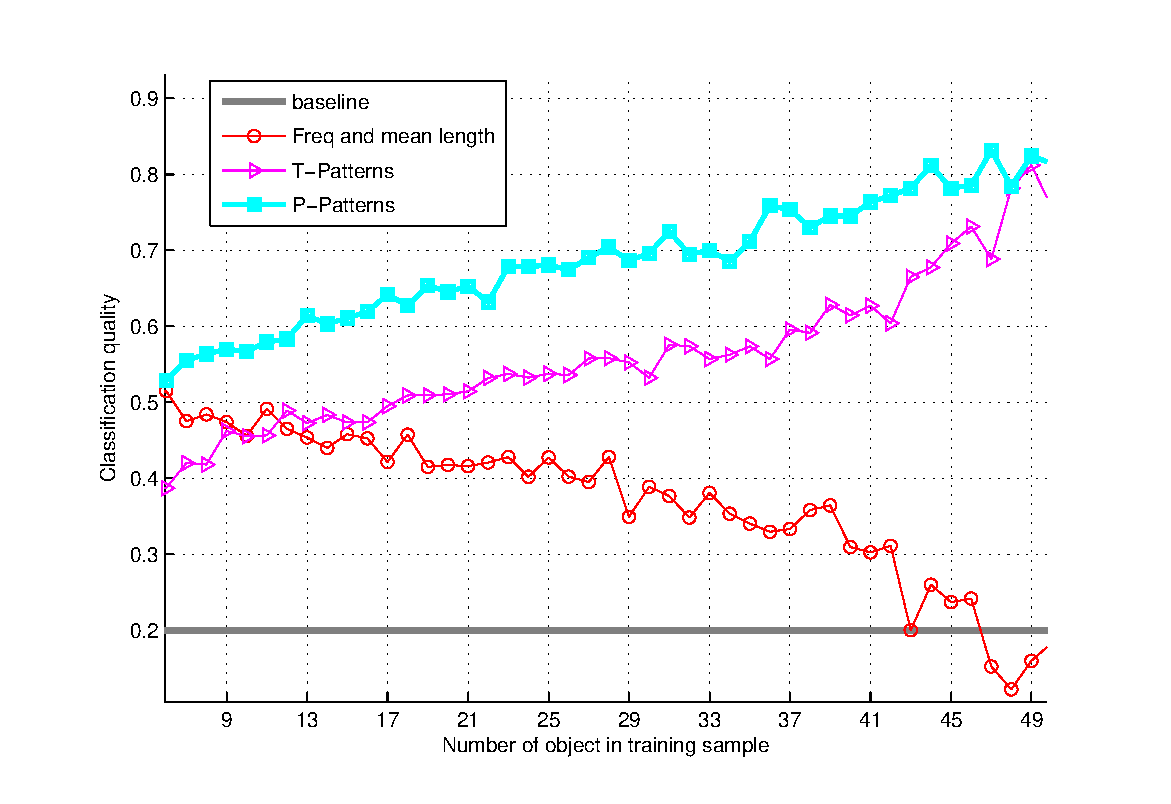
\includegraphics[width=173mm]{bad_data.eps}}
\caption{ Baseline означает, что приписывая метки класса случайно, можно получить, в среднем, такое качество классификации. Т.е. хуже некуда. 
Качество~--- средняя доля правильных классификаций.
По горизонтали откладывалось количество объектов в обучении(для каждого значение качество усреднялось по ста повторениям с разными разбиениями для обучения). }
\end{figure}
Очевидно(Рис. 1), что когда мы так специально добавили шумовую группу, классификация по длине и частоте актов становится крайне некачественная. 
При использовании паттернов, качество намного лучше, причем предложенные P-Паттерны обходят Т-Паттерны.

При рассмотрении confusion matrix ситуация еще более наглядная. На пересечении $i$-ой строки с
$j$-ым столбцом confusion matrix стоит число объектов $i$-го класса, отнесенного к $j$-ому классу. Таким образом,
у идеальной классификации confusion matrix должна иметь все нулевые элементы, кроме диагональных.

\begin{table}
\noindent
\label{tab:conft}
\begin{multicols}{2}
\noindent
\vfill
\hfill
\begin{tabular}{|c|c|c|c|c|c| }
\hline
~&1 & 2 & 3 & 4 & 5 \\
\hline
1 & 0.189 &   0.022 &   0.062  &  0.021  &  0.0007\\ \hline
2 & 0.015 &   0.083 &   0.015  &  0.079  &  0.001\\ \hline
3 & 0.014 &   0.014 &   0.113  &  0.051  &  0.001\\ \hline
4 & 0.001 &   0.035 &   0.011  &  0.144  &  0.003\\ \hline
5 & 0      &   0      &   0       &  0       &  0.116\\ \hline
\end{tabular}
\vfill
\hfill
\begin{tabular}{|c|c|c|c|c|c| }
\hline
~&1 & 2 & 3 & 4 & 5 \\
\hline
1 & 0.073  &  0.003 &   0.213 &   0.003 &        0\\ \hline
2 & 0.014  &  0.065 &   0.010 &   0.106 &        0\\ \hline
3 & 0.093  &  0.003 &   0.092 &   0.003 &        0\\ \hline
4 & 0.015  &  0.102 &   0.012 &   0.068 &        0\\ \hline
5 & 0.004  &  0.008 &   0.002 &   0.007 &   0.095\\ \hline
\end{tabular}
\end{multicols}
\caption{Слева: нормированная confusion matrix для классификации по P-Паттернам, справа: по частотам и средним продолжительностям.}
\end{table}


\begin{figure}[H]
\label{fig:conff}
	\begin{multicols}{2}
	\hfill
	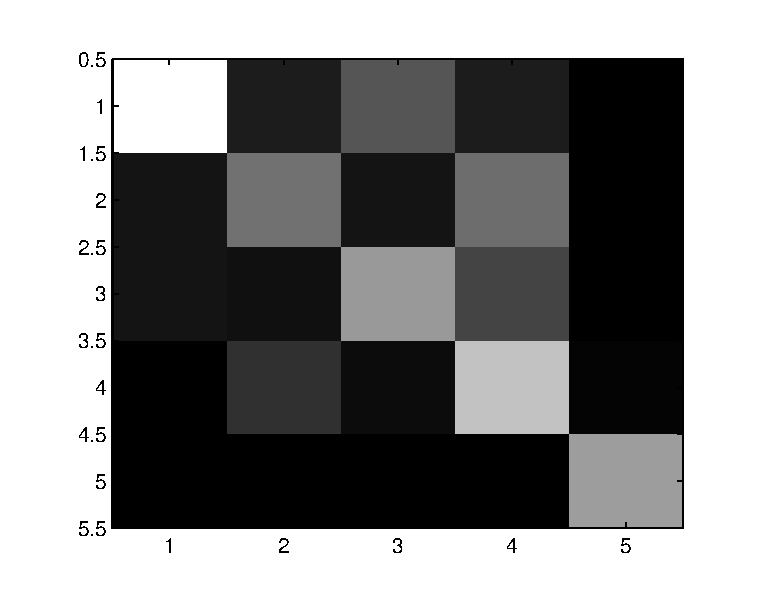
\includegraphics[width=90mm]{confusion_Ppat.eps}

	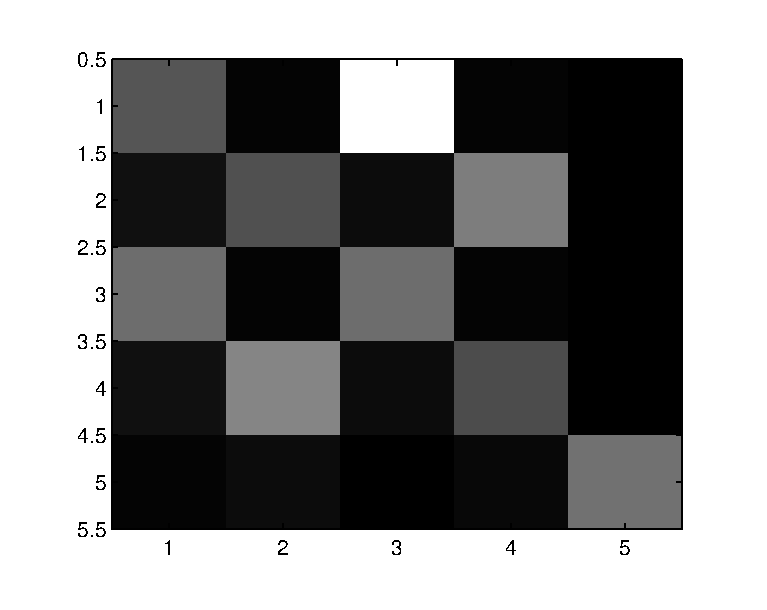
\includegraphics[width=90mm]{confusion_freq.eps}
	\end{multicols}
	\caption{Слева: confusion matrix для классификации по P-Паттернам, справа: по частотам и средним продолжительностям.}
\label{fig:omp_tp}
\end{figure}

На наших данных видно(Таб. 1, Рис. 2), что как и следовало ожидать, метод 1
сильно перепутывает 1-ый класс с 3-им, а 2-ой с 4-ым(методы поиска паттернов тоже перепутывают, но намного меньше). 
Отметим, что методы 2 и 3 могу перепутать 3-ий класс с 4-ым,
так как там вообще шум и бессмысленно требовать разделимость шума по паттернам. Тем не менее, для
нашего метода матрица намного ближе к диагональной.

В общем, был приведен пример зашумленных реальных данных, где для классификации наш метод работает лучше существующих.
было бы интересно узнать, существуют ли в поведении такие задачи. 
\section{Комментарий}
Здесь паттерны использовались, как некоторый <<мешок слов>>(это достаточно формализованное понятие в области машинного обучения~--- bag of words), 
мы смотрим, как <<откликается>>(каким образом паттерн входит в поведение) входной файл на каждый паттерн из этого мешка и так получаем 
вектор признаков.  Таким образом здесь паттерны создают нам некоторую статистику, нам не особо то важен вид каждого отдельного паттерна.
Оценить работу метода именно как инструмент поиска конкретных паттернов можно дать после встречи с Ириной. 
\newpage
\end{document}
